% Options for packages loaded elsewhere
\PassOptionsToPackage{unicode}{hyperref}
\PassOptionsToPackage{hyphens}{url}
\PassOptionsToPackage{dvipsnames,svgnames,x11names}{xcolor}
%
\documentclass[
  letterpaper,
  DIV=11,
  numbers=noendperiod]{scrreprt}

\usepackage{amsmath,amssymb}
\usepackage{lmodern}
\usepackage{iftex}
\ifPDFTeX
  \usepackage[T1]{fontenc}
  \usepackage[utf8]{inputenc}
  \usepackage{textcomp} % provide euro and other symbols
\else % if luatex or xetex
  \usepackage{unicode-math}
  \defaultfontfeatures{Scale=MatchLowercase}
  \defaultfontfeatures[\rmfamily]{Ligatures=TeX,Scale=1}
\fi
% Use upquote if available, for straight quotes in verbatim environments
\IfFileExists{upquote.sty}{\usepackage{upquote}}{}
\IfFileExists{microtype.sty}{% use microtype if available
  \usepackage[]{microtype}
  \UseMicrotypeSet[protrusion]{basicmath} % disable protrusion for tt fonts
}{}
\makeatletter
\@ifundefined{KOMAClassName}{% if non-KOMA class
  \IfFileExists{parskip.sty}{%
    \usepackage{parskip}
  }{% else
    \setlength{\parindent}{0pt}
    \setlength{\parskip}{6pt plus 2pt minus 1pt}}
}{% if KOMA class
  \KOMAoptions{parskip=half}}
\makeatother
\usepackage{xcolor}
\setlength{\emergencystretch}{3em} % prevent overfull lines
\setcounter{secnumdepth}{5}
% Make \paragraph and \subparagraph free-standing
\ifx\paragraph\undefined\else
  \let\oldparagraph\paragraph
  \renewcommand{\paragraph}[1]{\oldparagraph{#1}\mbox{}}
\fi
\ifx\subparagraph\undefined\else
  \let\oldsubparagraph\subparagraph
  \renewcommand{\subparagraph}[1]{\oldsubparagraph{#1}\mbox{}}
\fi

\usepackage{color}
\usepackage{fancyvrb}
\newcommand{\VerbBar}{|}
\newcommand{\VERB}{\Verb[commandchars=\\\{\}]}
\DefineVerbatimEnvironment{Highlighting}{Verbatim}{commandchars=\\\{\}}
% Add ',fontsize=\small' for more characters per line
\usepackage{framed}
\definecolor{shadecolor}{RGB}{241,243,245}
\newenvironment{Shaded}{\begin{snugshade}}{\end{snugshade}}
\newcommand{\AlertTok}[1]{\textcolor[rgb]{0.68,0.00,0.00}{#1}}
\newcommand{\AnnotationTok}[1]{\textcolor[rgb]{0.37,0.37,0.37}{#1}}
\newcommand{\AttributeTok}[1]{\textcolor[rgb]{0.40,0.45,0.13}{#1}}
\newcommand{\BaseNTok}[1]{\textcolor[rgb]{0.68,0.00,0.00}{#1}}
\newcommand{\BuiltInTok}[1]{\textcolor[rgb]{0.00,0.23,0.31}{#1}}
\newcommand{\CharTok}[1]{\textcolor[rgb]{0.13,0.47,0.30}{#1}}
\newcommand{\CommentTok}[1]{\textcolor[rgb]{0.37,0.37,0.37}{#1}}
\newcommand{\CommentVarTok}[1]{\textcolor[rgb]{0.37,0.37,0.37}{\textit{#1}}}
\newcommand{\ConstantTok}[1]{\textcolor[rgb]{0.56,0.35,0.01}{#1}}
\newcommand{\ControlFlowTok}[1]{\textcolor[rgb]{0.00,0.23,0.31}{#1}}
\newcommand{\DataTypeTok}[1]{\textcolor[rgb]{0.68,0.00,0.00}{#1}}
\newcommand{\DecValTok}[1]{\textcolor[rgb]{0.68,0.00,0.00}{#1}}
\newcommand{\DocumentationTok}[1]{\textcolor[rgb]{0.37,0.37,0.37}{\textit{#1}}}
\newcommand{\ErrorTok}[1]{\textcolor[rgb]{0.68,0.00,0.00}{#1}}
\newcommand{\ExtensionTok}[1]{\textcolor[rgb]{0.00,0.23,0.31}{#1}}
\newcommand{\FloatTok}[1]{\textcolor[rgb]{0.68,0.00,0.00}{#1}}
\newcommand{\FunctionTok}[1]{\textcolor[rgb]{0.28,0.35,0.67}{#1}}
\newcommand{\ImportTok}[1]{\textcolor[rgb]{0.00,0.46,0.62}{#1}}
\newcommand{\InformationTok}[1]{\textcolor[rgb]{0.37,0.37,0.37}{#1}}
\newcommand{\KeywordTok}[1]{\textcolor[rgb]{0.00,0.23,0.31}{#1}}
\newcommand{\NormalTok}[1]{\textcolor[rgb]{0.00,0.23,0.31}{#1}}
\newcommand{\OperatorTok}[1]{\textcolor[rgb]{0.37,0.37,0.37}{#1}}
\newcommand{\OtherTok}[1]{\textcolor[rgb]{0.00,0.23,0.31}{#1}}
\newcommand{\PreprocessorTok}[1]{\textcolor[rgb]{0.68,0.00,0.00}{#1}}
\newcommand{\RegionMarkerTok}[1]{\textcolor[rgb]{0.00,0.23,0.31}{#1}}
\newcommand{\SpecialCharTok}[1]{\textcolor[rgb]{0.37,0.37,0.37}{#1}}
\newcommand{\SpecialStringTok}[1]{\textcolor[rgb]{0.13,0.47,0.30}{#1}}
\newcommand{\StringTok}[1]{\textcolor[rgb]{0.13,0.47,0.30}{#1}}
\newcommand{\VariableTok}[1]{\textcolor[rgb]{0.07,0.07,0.07}{#1}}
\newcommand{\VerbatimStringTok}[1]{\textcolor[rgb]{0.13,0.47,0.30}{#1}}
\newcommand{\WarningTok}[1]{\textcolor[rgb]{0.37,0.37,0.37}{\textit{#1}}}

\providecommand{\tightlist}{%
  \setlength{\itemsep}{0pt}\setlength{\parskip}{0pt}}\usepackage{longtable,booktabs,array}
\usepackage{calc} % for calculating minipage widths
% Correct order of tables after \paragraph or \subparagraph
\usepackage{etoolbox}
\makeatletter
\patchcmd\longtable{\par}{\if@noskipsec\mbox{}\fi\par}{}{}
\makeatother
% Allow footnotes in longtable head/foot
\IfFileExists{footnotehyper.sty}{\usepackage{footnotehyper}}{\usepackage{footnote}}
\makesavenoteenv{longtable}
\usepackage{graphicx}
\makeatletter
\def\maxwidth{\ifdim\Gin@nat@width>\linewidth\linewidth\else\Gin@nat@width\fi}
\def\maxheight{\ifdim\Gin@nat@height>\textheight\textheight\else\Gin@nat@height\fi}
\makeatother
% Scale images if necessary, so that they will not overflow the page
% margins by default, and it is still possible to overwrite the defaults
% using explicit options in \includegraphics[width, height, ...]{}
\setkeys{Gin}{width=\maxwidth,height=\maxheight,keepaspectratio}
% Set default figure placement to htbp
\makeatletter
\def\fps@figure{htbp}
\makeatother
\newlength{\cslhangindent}
\setlength{\cslhangindent}{1.5em}
\newlength{\csllabelwidth}
\setlength{\csllabelwidth}{3em}
\newlength{\cslentryspacingunit} % times entry-spacing
\setlength{\cslentryspacingunit}{\parskip}
\newenvironment{CSLReferences}[2] % #1 hanging-ident, #2 entry spacing
 {% don't indent paragraphs
  \setlength{\parindent}{0pt}
  % turn on hanging indent if param 1 is 1
  \ifodd #1
  \let\oldpar\par
  \def\par{\hangindent=\cslhangindent\oldpar}
  \fi
  % set entry spacing
  \setlength{\parskip}{#2\cslentryspacingunit}
 }%
 {}
\usepackage{calc}
\newcommand{\CSLBlock}[1]{#1\hfill\break}
\newcommand{\CSLLeftMargin}[1]{\parbox[t]{\csllabelwidth}{#1}}
\newcommand{\CSLRightInline}[1]{\parbox[t]{\linewidth - \csllabelwidth}{#1}\break}
\newcommand{\CSLIndent}[1]{\hspace{\cslhangindent}#1}

\KOMAoption{captions}{tableheading}
\makeatletter
\makeatother
\makeatletter
\@ifpackageloaded{bookmark}{}{\usepackage{bookmark}}
\makeatother
\makeatletter
\@ifpackageloaded{caption}{}{\usepackage{caption}}
\AtBeginDocument{%
\ifdefined\contentsname
  \renewcommand*\contentsname{Table of contents}
\else
  \newcommand\contentsname{Table of contents}
\fi
\ifdefined\listfigurename
  \renewcommand*\listfigurename{List of Figures}
\else
  \newcommand\listfigurename{List of Figures}
\fi
\ifdefined\listtablename
  \renewcommand*\listtablename{List of Tables}
\else
  \newcommand\listtablename{List of Tables}
\fi
\ifdefined\figurename
  \renewcommand*\figurename{Figure}
\else
  \newcommand\figurename{Figure}
\fi
\ifdefined\tablename
  \renewcommand*\tablename{Table}
\else
  \newcommand\tablename{Table}
\fi
}
\@ifpackageloaded{float}{}{\usepackage{float}}
\floatstyle{ruled}
\@ifundefined{c@chapter}{\newfloat{codelisting}{h}{lop}}{\newfloat{codelisting}{h}{lop}[chapter]}
\floatname{codelisting}{Listing}
\newcommand*\listoflistings{\listof{codelisting}{List of Listings}}
\makeatother
\makeatletter
\@ifpackageloaded{caption}{}{\usepackage{caption}}
\@ifpackageloaded{subcaption}{}{\usepackage{subcaption}}
\makeatother
\makeatletter
\@ifpackageloaded{tcolorbox}{}{\usepackage[many]{tcolorbox}}
\makeatother
\makeatletter
\@ifundefined{shadecolor}{\definecolor{shadecolor}{rgb}{.97, .97, .97}}
\makeatother
\makeatletter
\makeatother
\ifLuaTeX
  \usepackage{selnolig}  % disable illegal ligatures
\fi
\IfFileExists{bookmark.sty}{\usepackage{bookmark}}{\usepackage{hyperref}}
\IfFileExists{xurl.sty}{\usepackage{xurl}}{} % add URL line breaks if available
\urlstyle{same} % disable monospaced font for URLs
\hypersetup{
  pdftitle={EDLD 710: Data Analysis for Problems of Practice},
  pdfauthor={Jack B. Huber, Ph.D.},
  colorlinks=true,
  linkcolor={blue},
  filecolor={Maroon},
  citecolor={Blue},
  urlcolor={Blue},
  pdfcreator={LaTeX via pandoc}}

\title{EDLD 710: Data Analysis for Problems of Practice}
\author{Jack B. Huber, Ph.D.}
\date{2022-08-31T08:46:51-07:00}

\begin{document}
\maketitle
\ifdefined\Shaded\renewenvironment{Shaded}{\begin{tcolorbox}[interior hidden, frame hidden, enhanced, sharp corners, borderline west={3pt}{0pt}{shadecolor}, boxrule=0pt, breakable]}{\end{tcolorbox}}\fi

\renewcommand*\contentsname{Table of contents}
{
\hypersetup{linkcolor=}
\setcounter{tocdepth}{2}
\tableofcontents
}
\bookmarksetup{startatroot}

\hypertarget{purpose-of-this-document}{%
\chapter*{Purpose of this Document}\label{purpose-of-this-document}}
\addcontentsline{toc}{chapter}{Purpose of this Document}

The purpose of this site\footnote{This site was built in \texttt{R}
  (\textbf{R-base?}) with \texttt{R\ Markdown} (\textbf{R-rmarkdown?}).}
is to offer targeted advice and resources to help you analyze the
quantitative data you have collected for your capstone project.

The chapter structure to the left illustrates the organization of this
site. Each page attempts to identify and deal with important issues that
come up in the process on analyzing quantitative data. This includes
explanation, advice, and links to resources where available and
appropriate.

These pages are works in progress. The intent is for them to evolve in
adaptation to your needs. I will continue to edit them as I see fit; and
if something is missing, please don't hesitate to reach out to me:
\href{mailto:huberj@gonzaga.edu}{\nolinkurl{huberj@gonzaga.edu}}.\footnote{A
  little bit \href{AboutMe.html}{about me}\href{Projects.html}{.}}

\bookmarksetup{startatroot}

\hypertarget{preparing-your-data}{%
\chapter*{Preparing your Data}\label{preparing-your-data}}
\addcontentsline{toc}{chapter}{Preparing your Data}

The purpose of this page is to help you clean, organize, and otherwise
prepare and enhance your data for statistical analysis and/or
visualization.

\begin{center}\rule{0.5\linewidth}{0.5pt}\end{center}

\hypertarget{best-practices-for-excel}{%
\section*{Best practices for Excel}\label{best-practices-for-excel}}
\addcontentsline{toc}{section}{Best practices for Excel}

In all likelihood the primary tool you'll use for working with your data
is Excel - possibly by now the most commonly used tool for working with
data in the world. What follows is a list of good practices that might
make your Excel data easier to manage and collaborate with others. These
tips will save you time wasted on fixing data and will help keep your
data in format appropriate for analysis:

\textbf{Put \emph{variables in columns} and \emph{observations in
rows}}. Include a unique identifying number for each case. Be sure that
each variable name is unique (no duplicate variable names).

\textbf{Put \emph{variable names} in the \emph{first row}}. Variables
must start with a letter. Do not include special characters (\#, !, ?,
\%, etc.) or spaces in your variable names.

\textbf{Keep all your data ``touching''. \emph{No empty rows or
columns}}. This is critically important for sorting. Empty columns or
rows break the structural integrity of your data set and could allow you
to sort a subsection of your data apart the rest of it.

\textbf{No merged cells}.

\textbf{Use a separate column for each piece of information}. Don't
enter data such as ``120/80'' for blood pressure. Enter systolic blood
pressure as one variable and diastolic blood pressure as another
variable. Don't enter data as ``A,C,D'' or ``BDF'' if there are three
possible answers to a question. Include a separate column for each
answer.

\textbf{Decide on a ``missingness'' convention}. Missing data can cause
a multitude of problems. To enter a missing data value either enter a
blank or an ``impossible'' numeric code (for numbers) or an easily
recognizable single digit character code for character (trying to avoid
mixing numeric and character data). Be sure, if you use a missing value
code, that it cannot be confused with a ``real'' data value.

\textbf{Use only one worksheet for your data; do analysis on a different
worksheet}. If you decide to use multiple sheets for you data, follow
the variable naming conventions for the tabs that name the sheets (keep
the names simple and unique).

\textbf{Do not ``stack'' data on the same sheets}. For example,
``treated'' versus ``non-treated'' patients can be handled by column
variable that has a code for Treated (yes/no).

\textbf{Dedicate one worksheet to your original, unedited raw data. Make
a copy of it to do all your cleaning and analysis}. You might label this
worksheet ``Original'' or ``Raw data.'' This is important so that
\textbf{when you make a mistake, you always have your original data to
fall back on}.

\textbf{Dedicate one worksheet to your Clean / Working data}.

\textbf{Make the most of your variable labels}. On your worksheet of
``Clean'' (or ``Working'') data, make sure every column of data has a
clear, concise, descriptive label. Here's what I do to take column
labels to the next level:

\begin{itemize}
\tightlist
\item
  Ensure that the top row of my data includes a clear, concise label for
  each column of data.
\item
  Bold the row.
\item
  Add a fill color to the row.
\item
  Freeze the row (Select the row, then View --\textgreater{} Freeze top
  row).
\item
  Enable word wrap in the row.
\end{itemize}

\textbf{Apply a consistent format for your columns}. Data elements are
different sizes. Names tend to be long while numerical values tend to be
short. I don't like it when a column label is left-aligned but the data
are right-aligned. I find these variations in visual formatting
distracting. To deal with these distractions, I tend to:

\begin{itemize}
\tightlist
\item
  Apply all the column label formatting mentioned above.
\item
  Fix all my column widths to 15.
\item
  Left align columns (both column labels and data) for text (patient
  names, medication names, etc.).
\item
  Center columns (both column labels and data) for numeric values.
\item
  Right align columns for time data.
\end{itemize}

I find (and I think you will too) that enforcing a consistent format
removes variable formatting as a distraction so I can see and focus on
the data.

\begin{center}\rule{0.5\linewidth}{0.5pt}\end{center}

\hypertarget{excel-skills}{%
\section*{Excel skills}\label{excel-skills}}
\addcontentsline{toc}{section}{Excel skills}

Here are the skills you will most likely need and use:

\begin{itemize}
\tightlist
\item
  Sorting your data array on a column
\item
  Filtering your data array based on specific values of one or more
  columns
\item
  Fill down
\item
  Pivot Table
\item
  VLOOKUP function - to matching together related data from different
  sources
\item
  Conditional formatting
\item
  Basic calculations (SUM, AVG, COUNTIF, etc.)
\item
  CONCATENATE function - to stitch together text and values from
  different data columns into a new column (which is sometimes helpful
  and necessary but is generally bad data practice to be avoided)
\end{itemize}

\begin{center}\rule{0.5\linewidth}{0.5pt}\end{center}

\hypertarget{resources-for-data-preparation}{%
\section*{Resources for data
preparation}\label{resources-for-data-preparation}}
\addcontentsline{toc}{section}{Resources for data preparation}

\href{https://vita.had.co.nz/papers/tidy-data.pdf}{Tidy Data}, by Hadley
Wickham (a well-known data scientist), is a classic paper that defines
what makes data clean (or ``tidy'') {[}@WickhamTidy{]}

The University of New Hampshire Library has an excellent
\href{https://libraryguides.unh.edu/excel}{research guide for using
Excel}, including
\href{https://libraryguides.unh.edu/excel/cleaning}{data cleaning},
\href{https://libraryguides.unh.edu/excel/analysis}{data analysis},
\href{https://libraryguides.unh.edu/excel/visualization}{data
visualization}, and
\href{https://libraryguides.unh.edu/excel/bestpractices}{spreadsheet
best practices}.

\href{https://libraryguides.unh.edu/excel/bestpractices}{Preparing Data
in Excel}, from the University of Nebraska Medical Center College of
Public Health, has an excellent set of guidelines for working with Excel

\href{https://lo.unisa.edu.au/mod/book/view.php?id=646440\&chapterid=164660}{Introduction
to Excel} is an excellent online module from the University of South
Australia Research Methodologies and Statistics department.

\href{https://datamanagement.hms.harvard.edu/analyze/analysis-ready-datasets}{Analysis
Ready Datasets} is an excellent resource from Harvard Medical School

\begin{center}\rule{0.5\linewidth}{0.5pt}\end{center}

\hypertarget{granularity-of-data}{%
\section*{Granularity of data}\label{granularity-of-data}}
\addcontentsline{toc}{section}{Granularity of data}

Granularity of data means two related things worth your attention:

\begin{enumerate}
\def\labelenumi{\arabic{enumi}.}
\item
  One is the \emph{size of the data point}, which is to say what context
  it provides for other, smaller, data points. Put another way, what
  data points do you intend to count or summarize, and by which groups
  do you intend to compare these summaries?
\item
  The other is, essentially this question: What does a \emph{row} in the
  spreadsheet mean? Because Excel counts rows, but what's contained in a
  row may not be what you intend to count.
\end{enumerate}

Here are several different levels of granularity of Epic data:

\textbf{Patient level}. A patient has a unique ID number: the MRN. No
two patients have the same MRN. When it comes to mining Epic data for
the research project, the patient list is perhaps the most important:
the resident needs a ``patient list''. When it comes to data mining, the
patient ``level'' is context to more granular data in the sense that a
patient can have multiple encounters - and thus multiple Encounter CSNs
``within'' the same Patient MRN.

\textbf{Encounter level}. The unique Epic ID number for the encounter is
the CSN. The encounter is context to more granular data such as a
treatment regimen of a particular medicine. Multiple drug
administrations can occur ``within'' an encounter CSN.

\textbf{Medication administration level}. This is possibly the lowest
level and the most granular data. In Caboodle, each administration of a
medicine has a unique ID number and is time-stamped. My queries to date
have been for counts of medicine administrations, or firsts, lasts,
minimums and maximum doses within a hospital encounter or ICU stay.

\textbf{Lab results level}. Lab data is similar to medicine
administration data because, again in Caboodle, each lab result is has
its own unique ID number and is time-stamped. There can be a great many
lab results within a hospital encounter. My queries to date have been
for counts of lab results, or firsts, lasts, minimums and maximum values
within a hospital encounter or ICU stay.

The resident data collection form is designed for patient level data;
each row in the spreadsheet captures the experience of a hospital
encounter. It can also be helpful to report the medicine administration
and lab result data sorted chronologically by patient and encounter.

\bookmarksetup{startatroot}

\hypertarget{analyzing-your-data}{%
\chapter*{Analyzing your Data}\label{analyzing-your-data}}
\addcontentsline{toc}{chapter}{Analyzing your Data}

The purpose of this page is to give you tools to analyze your data using
appropriate statistics. There are two important tasks:

\begin{enumerate}
\def\labelenumi{\arabic{enumi}.}
\tightlist
\item
  Define the measurement levels of your variables.
\item
  Choose statistics appropriate for the measurement levels of your
  variables and the purpose of your analysis.
\end{enumerate}

\begin{center}\rule{0.5\linewidth}{0.5pt}\end{center}

\hypertarget{define-the-measurement-levels-of-your-variables}{%
\section*{Define the measurement levels of your
variables}\label{define-the-measurement-levels-of-your-variables}}
\addcontentsline{toc}{section}{Define the measurement levels of your
variables}

It is important to know the measurement level of your variables (De Muth
2009). How do you express the outcome by which to compare your pre- and
post- samples? Is it\ldots{}

\begin{itemize}
\tightlist
\item
  Percent of patients who achieve an initial therapeutic goal?
\item
  Time to initial therapeutic level?
\item
  Percent of patients who experience an adverse outcome (such as acute
  kidney injury)?
\item
  Mortality rate (\% surviving)? In such a case you would be comparing
  two proportions.
\item
  ``Time to\ldots{}'' a therapeutic level? In such a case you would be
  comparing two different quantities of time.
\end{itemize}

\hypertarget{nominal-measurement}{%
\subsection*{Nominal measurement}\label{nominal-measurement}}
\addcontentsline{toc}{subsection}{Nominal measurement}

Nominal measurement is categories. Each patient must fall into only one
category, and the categories must be mutually exclusive and exhaustive.
Here are some examples:

\begin{itemize}
\tightlist
\item
  Gender (Male/Female)
\item
  Racial identity
\item
  Marital status
\item
  Control group/Experimental group
\item
  Infected with COVID vs.~not infected with COVID
\item
  Disease presence
\item
  Mortality
\end{itemize}

Outcomes are usually reported as frequency counts or percentages (in
each category).

\hypertarget{ordinal-measurement}{%
\subsection*{Ordinal measurement}\label{ordinal-measurement}}
\addcontentsline{toc}{subsection}{Ordinal measurement}

Ordinal measure also puts patients into categories, but the categories
have an ascending or descending order: patients have \emph{more} or
\emph{less} of somthing. But the differences between the categories is
not necessarily the same. Here are some examples:

\begin{itemize}
\tightlist
\item
  Stages I-IV tumors
\item
  0-10 Apgar scores
\end{itemize}

A Stage IV tumor is more advanced than a Stage II tumor, but not
necessarily by twice as much. A Stage III tumor is more advanced than a
Stage I tumor, but not necessarily by three times as much.

For this reason, we cannot perform arithmetic or calculate means or
other parametric statistics on ordinal values.

However, if your project has an ordinal level outcome on which you need
to compare treatment groups, there are appropriate
\textbf{nonparametric} statistics you can use to see which group is
significantly \emph{more of} this outcome than another. Examples
include:

\begin{itemize}
\tightlist
\item
  \textbf{chi-square} \(\chi 2\) statistics
\item
  the \textbf{Mann-Whitney U} test
\item
  the \textbf{Spearman's rho} test
\end{itemize}

\hypertarget{interval-and-ratio-level-measurement}{%
\subsection*{Interval and ratio level
measurement}\label{interval-and-ratio-level-measurement}}
\addcontentsline{toc}{subsection}{Interval and ratio level measurement}

Finally, interval and ratio measurement means \textbf{continuous} data:
patients fall somewhere on a continuum, like a temperature scale. As a
result, variables measured using interval and ratio scales are often
referred to as continuous variables. Here are some examples:

\begin{itemize}
\tightlist
\item
  Height
\item
  Weight
\item
  Cholesterol level
\item
  Blood pressure
\item
  Time
\end{itemize}

On variables like these there is relative positioning with no gaps or
interruptions in the continuum.

The difference between interval and ratio scales is that ratio has a
true zero value while interval does not.

On variables like these it is permissible to do arithmetic and to
summarize them with the \textbf{mean} and \textbf{standard deviation}
which, in turn, avail to you more commonly used advanced statistics
like:

\begin{itemize}
\tightlist
\item
  t tests
\item
  analyses of variance (ANOVA)
\item
  correlation
\item
  regression
\end{itemize}

Once you have a good feel for the measurement levels of your outcome and
predictor variables, you can choose appropriate statistics.
(\textbf{Simpson2015?}) offers two decision trees to help you make these
choices:

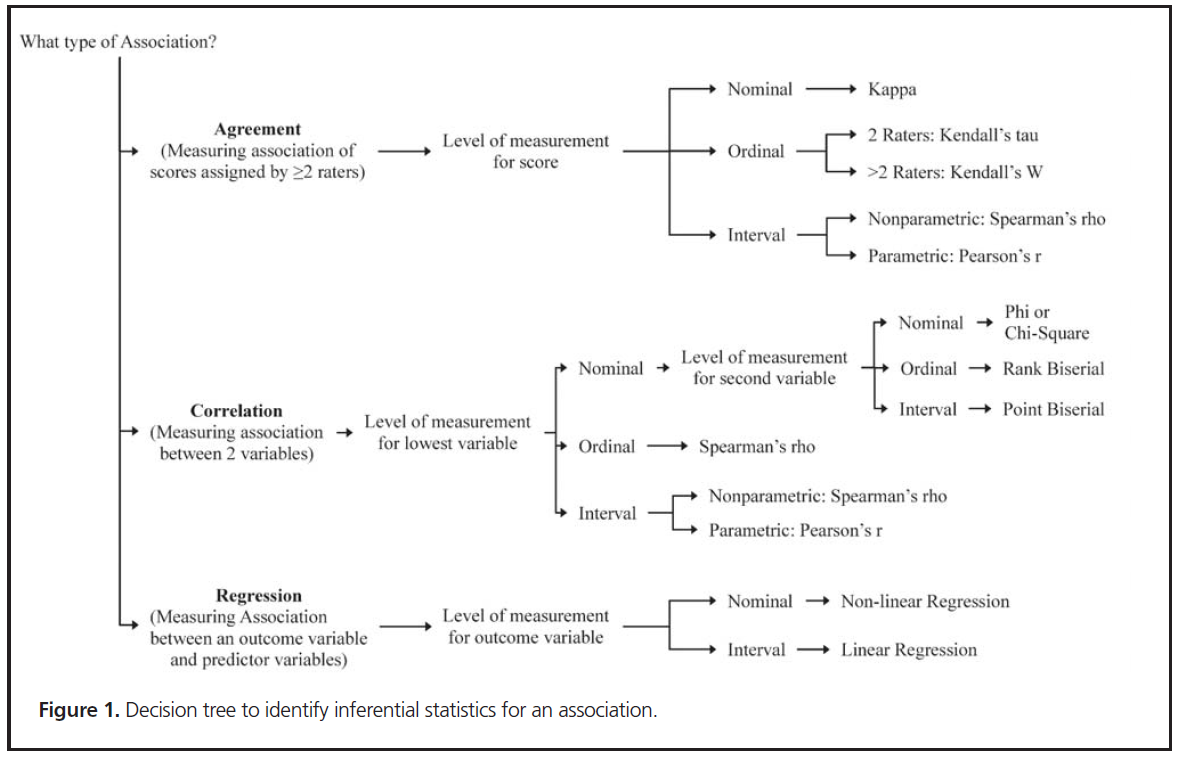
\includegraphics{./images/stat-tree-fig1.PNG}
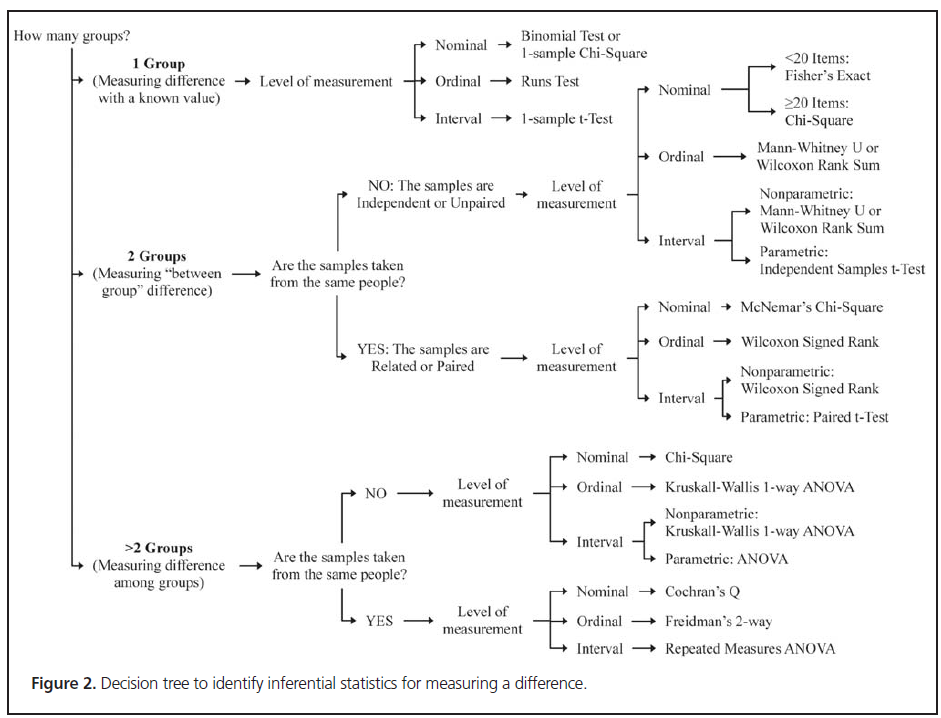
\includegraphics{./images/stat-tree-fig2.png}

\begin{center}\rule{0.5\linewidth}{0.5pt}\end{center}

\hypertarget{choose-appropriate-statistics}{%
\section*{Choose appropriate
statistics}\label{choose-appropriate-statistics}}
\addcontentsline{toc}{section}{Choose appropriate statistics}

This section offers more information on several choice statistics. These
are statistics I've used for recent resident projects and seen in the
journals.

\hypertarget{chi-square-chi-2-tests}{%
\subsection*{\texorpdfstring{Chi-square \(\chi 2\)
tests}{Chi-square \textbackslash chi 2 tests}}\label{chi-square-chi-2-tests}}
\addcontentsline{toc}{subsection}{Chi-square \(\chi 2\) tests}

The chi-square \(\chi 2\) test is a commonly used statistic for
nominal/categorical data. We use it to examine the distribution of cases
across \textbf{categories}. Essentially, it compares the distribution of
cases you actually see to the distribution of cases you would expect to
see from normal variation.

Here is one example of a chi-square \(\chi 2\) test for a recent
resident project. The question is whether gender (male/female) makes a
statistically significant difference in whether patients need three or
more dose changes of bivalirudin before they reach a therapeutic goal.

\begin{Shaded}
\begin{Highlighting}[]
\CommentTok{\#d \textless{}{-} read.csv("data/bivalirudin.csv") \# load data}
\CommentTok{\#table\_dosechgs\_gender \textless{}{-} xtabs(\textasciitilde{}d$d\_Male + d$DV\_3DoseChanges, data=d) \# crosstabulate }
\CommentTok{\#knitr::kable(table\_dosechgs\_gender, align = "l")}
\CommentTok{\#summary(table\_dosechgs\_gender) \# calculate chi{-}square}
\end{Highlighting}
\end{Shaded}

The chi-square \(\chi 2\) value of 1.9421 with one degree of freedom has
a p-value of 0.1634. It is not statistically significant, suggesting
that gender makes no significant difference in reaching therapeutic
goal.

\hypertarget{t-tests}{%
\subsection*{t tests}\label{t-tests}}
\addcontentsline{toc}{subsection}{t tests}

The t test is a commonly used statistic for comparing two groups on a
continuous outcome. Here are some examples of t tests from a recent
resident project:

propofol\_stats.xlsx

\begin{center}\rule{0.5\linewidth}{0.5pt}\end{center}

\hypertarget{external-resources-for-data-analysis}{%
\section*{External resources for data
analysis}\label{external-resources-for-data-analysis}}
\addcontentsline{toc}{section}{External resources for data analysis}

Here are a few links to external resources on data analysis and
statistics.

\begin{itemize}
\tightlist
\item
  \href{https://rpsychologist.com/}{The R Psychologist, by
  @magnussonCohend} - is an outstanding resource to better understand
  statistics
\item
  \href{https://lo.unisa.edu.au/course/view.php?id=8481}{Online Modules
  in Research Methods and Data Analysis} at the University of South
  Australia
\item
  \href{https://libraryguides.unh.edu/excel/analysis}{Data Analysis}
  from the University of New Hampshire
\end{itemize}

\begin{center}\rule{0.5\linewidth}{0.5pt}\end{center}

\hypertarget{software-tools-for-data-analysis}{%
\section*{Software tools for data
analysis}\label{software-tools-for-data-analysis}}
\addcontentsline{toc}{section}{Software tools for data analysis}

Of equal importance to the didactics of statistics are the brass tacks
of software for working with statistics. Here are several software tools
for analyzing data:

\hypertarget{excel-based-tools}{%
\subsection*{Excel-based tools}\label{excel-based-tools}}
\addcontentsline{toc}{subsection}{Excel-based tools}

\begin{itemize}
\tightlist
\item
  \href{http://www.ezanalyze.com/}{EZAnalyze} is a simple Excel add-in
  for data analysis. It includes menus for selecting various statistics
  from your variables.
\item
  \href{https://www.xlstat.com/en/}{XLStat}
\item
  Data Analysis native add-in
\end{itemize}

\hypertarget{data-analysis-software}{%
\subsection*{Data analysis software}\label{data-analysis-software}}
\addcontentsline{toc}{subsection}{Data analysis software}

\begin{itemize}
\tightlist
\item
  \href{https://www.r-project.org/}{R @R-base}, with
  \href{https://www.rstudio.com/}{RStudio} and
  \href{https://rmarkdown.rstudio.com/}{R Markdown}, is \textbf{free}
  open source software for data analysis, statistics, and data
  visualization. It is powerful and flexible but it does require ongoing
  learning of code because it is constantly evolving.
\end{itemize}

Here are several other robust software applications for data analysis
available to you. One or more of them may be free for you as a Gonzaga
student:

\begin{itemize}
\tightlist
\item
  \href{https://itconnect.uw.edu/uware/jmp/}{JMP} - JMP is a suite of
  software used for statistical analysis
\item
  \href{https://itconnect.uw.edu/uware/sas/}{SAS} - The SAS System is a
  comprehensive statistical software package from SAS Institute for data
  management, graphics, analysis, and presentation
\item
  \href{https://itconnect.uw.edu/uware/spss/}{SPSS} - IBM SPSS
  (Statistical Package for the Social Sciences) provides data and
  statistical analysis, file management capabilities, graphics and
  reporting features
\end{itemize}

\bookmarksetup{startatroot}

\hypertarget{reporting-your-data}{%
\chapter*{Reporting your Data}\label{reporting-your-data}}
\addcontentsline{toc}{chapter}{Reporting your Data}

The purpose of this final page is to help you decide how best to package
and present the results of your data analysis for a professional
audience.

\begin{center}\rule{0.5\linewidth}{0.5pt}\end{center}

\hypertarget{best-practices-for-figures-i.e.-graphs}{%
\section*{Best practices for figures
(i.e.~graphs)}\label{best-practices-for-figures-i.e.-graphs}}
\addcontentsline{toc}{section}{Best practices for figures (i.e.~graphs)}

``Figures should be accurate, clear, and concise. As with tables, the
figure with its title and legend should be understandable without undue
reference to the text.''\footnote{\href{https://academic.oup.com/amamanualofstyle/book/27941/chapter/207563838}{From
  the AMA Style Guide, Section 4.2 on Figures}}

\hypertarget{line-graphs-for-over-time-data}{%
\subsection*{1. Line graphs for over-time
data}\label{line-graphs-for-over-time-data}}
\addcontentsline{toc}{subsection}{1. Line graphs for over-time data}

Line graphs are the appropriate way to show change over time in one or a
few groups. Your x-axis (horizontal) should be time, and your y-axis
should be the quantity by which you want to see change over time. You
can use different lines for different groups.

\hypertarget{bar-graphs-for-group-comparisons.}{%
\subsection*{2. Bar graphs for group
comparisons.}\label{bar-graphs-for-group-comparisons.}}
\addcontentsline{toc}{subsection}{2. Bar graphs for group comparisons.}

The bar graph is the Swiss army knife of data visualization. It's useful
because it is so versatile. Bar graphs use size to compare different
quantities. Your y-axis is your quantity and on your x-axis you put your
group categories.

\hypertarget{save-the-pies-for-dessert}{%
\subsection*{3. Save the pies for
dessert}\label{save-the-pies-for-dessert}}
\addcontentsline{toc}{subsection}{3. Save the pies for dessert}

Pie graphs are a great way to visualize proportions - parts that make up
a whole. And, with a few nice colors, they're attractive. They're also
simple.

But they can be a pain to create - to get right visually. They also lose
their utility when you have more than a few categories. For this reason,
the AMA discourages the use of pie graphs:

If you do want to use a pie graph, my advice to you is to keep it
simple; use it only to show a few categories.

\begin{center}\rule{0.5\linewidth}{0.5pt}\end{center}

\hypertarget{best-practices-for-tables}{%
\section*{Best practices for tables}\label{best-practices-for-tables}}
\addcontentsline{toc}{section}{Best practices for tables}

Although data visualization has become all the rage, there is a still a
place at the table for tables (sorry - bad pun - I couldn't resist).
Tables remain a concise way to present a sizable amount of quantitative
data.

I encourage you to strive for your tables to meet this standard: ``A
properly designed and constructed table should be able to stand
independently, without requiring undue reference to the
text.''\footnote{\href{https://academic.oup.com/amamanualofstyle/book/27941/chapter/207563838}{From
  Section 4.1 Tables, in AMA Style Guide}}

I encourage you to review the section on tables in the APA Style Guide.

\begin{itemize}
\tightlist
\item
  What goes on the far left column?
\item
  How do I format the main column headings?
\item
  How do I report p-values?
\item
  How do I report my data?
\item
  How do I align things?
\end{itemize}

This article from (\textbf{MillerEtAl2020?}) illustrates how to present
a table that reports the results of a series of chi-square tests of the
differences between two groups (pre-implementation and
post-implementation) on categorical outcomes.

Notice that the authors showed the independent variable (intervention
group) as columns which enables us as readers to compare outcomes by
reading left to right.

\bookmarksetup{startatroot}

\hypertarget{references}{%
\chapter*{References}\label{references}}
\addcontentsline{toc}{chapter}{References}

\hypertarget{refs}{}
\begin{CSLReferences}{1}{0}
\leavevmode\vadjust pre{\hypertarget{ref-DeMuth2009}{}}%
De Muth, James E. 2009. {``Overview of Biostatistics Used in Clinical
Research.''} \emph{American Journal of Health-System Pharmacy} 66:
70--81.

\end{CSLReferences}



\end{document}
